\section{Module 2: Lecture 7\\Fourier Transforms properties and Fourier series example}

\subsection{Introduction}
 In this lecture, we will take a few examples of the calculation of the Fourier transform and then build upon the general properties of a Fourier transform like linearity, time shift, modulation and convolution. \\
Let us start with calculating the Fourier transform of a rectangular pulse.
\subsection{Fourier transform of a Rectangular Pulse}
Let the pulse be symmetric, with height equal to $A$, going from $-T/2$ to $T/2$ on the time axis. We call this function h(t) or x(t) any one of them as shown in figure below.
%~\ref{rectangular_pulse}.

\begin{figure}[htp]
\centering
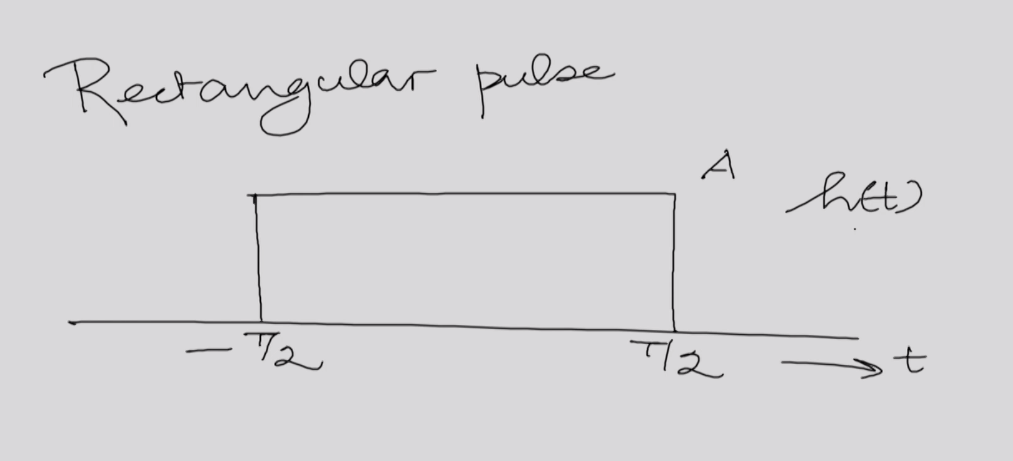
\includegraphics[width=12cm]{rectangularpulse.png}
\caption{Symmetric Rectangular Pulse}
\label{rectangular_pulse}
\end{figure}

Let us denote the Fourier transform by $ H(\Omega)$. Then

\begin{equation}
H(\Omega)=\int_{-\infty}^{\infty}{h(t) e^{-j\Omega t}}dt
\end{equation}

As h(t) is zero except in the time interval $-T/2$ to $T/2$, we can write the above equation as

\begin{equation}
H(\Omega)=\int_{-T/2}^{T/2}{A e^{-j\Omega t}}dt =
\frac{A e^{-j\Omega t}}{-j \Omega} \Bigg|_{-T/2}^{T/2}=
\frac{A(e^{-j\Omega T/2}-e^{j\Omega T/2})}{-j\Omega}
=\frac{AT (2j\sin({\Omega T/2}))}{j\Omega T}
\end{equation}

\begin{equation}
H(\Omega)=\frac{AT\sin({\Omega T/2})}{\Omega T/2}
\end{equation}
And we can rewrite it as

\begin{equation}
H(f)=\frac{AT \sin({2\pi f T/2})}{2\pi f T/2}
\end{equation}


Where $f = \cfrac{\Omega}{2\pi}$ corresponds to the ${cycles}/{second}$ frequency, and $\Omega$ is of course the angular frequency.

Now this expression also can be written as
\begin{equation}
H(\gamma)=\frac{AT \sin({\pi \gamma})}{\pi \gamma}
\end{equation}
Where $\gamma = f*T $

The function $\cfrac{\sin{\pi \gamma}}{\pi \gamma}$ is a very special function called a \emph{Sinc Function}. The sinc function in the form presented is often used in the context of signals and systems.

\subsubsection{Sketch of the Sinc function}

Here are the some properties of the Sinc function.
\begin{itemize}
\item It is an even function.
\item It has nulls at every integer; so at 1, at 2, at 3 and so on, it will have value equal to zero.
\item It tends to 1 as $\gamma$ tends to 0
\item It is a damped sinusoid, i.e. the magnitude of oscillation decreases as $\gamma$ increases.
\end{itemize}

Using the above points we can sketch the Sinc function. So the sketch somewhat looks like the figure below.
%~\ref{sinc}.

\begin{figure}[htp]
\centering
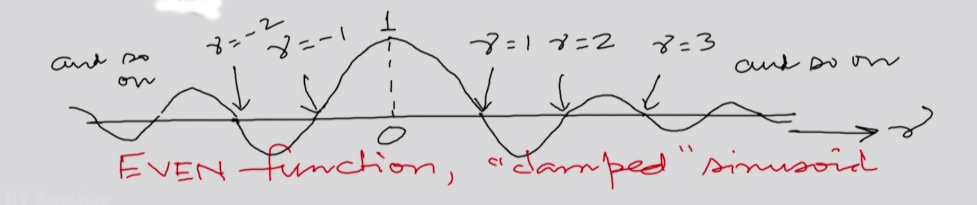
\includegraphics[width=12cm]{sinc.png}
\caption{Sinc Function}
\label{sinc}
\end{figure}

\subsubsection{Important points regarding the Fourier transform of rectangular pulse}


The pulse is limited in terms of its occupancy of the time axis. It goes only from  $-T/2$ to $+T/2$. On the other hand, the Fourier transform, in principle, last all over the frequency axis.
What this means is that if we want to make a function vanish all over the time axis outside a certain finite interval, we have to bring together frequencies of all magnitudes and signs except for a few nulls.
All these frequencies need to come together, in appropriate amplitudes, to form this rectangular pulse. Also note that the Fourier transform for this case is purely real. \\
 When the pulse width is halved, the nulls of the Fourier transform are doubly spaced and the central amplitude is halved. This can be checked mathematically. We can see that in the figure below.
%~\ref{pulse_FT_half}

\begin{figure}[htp]
\centering
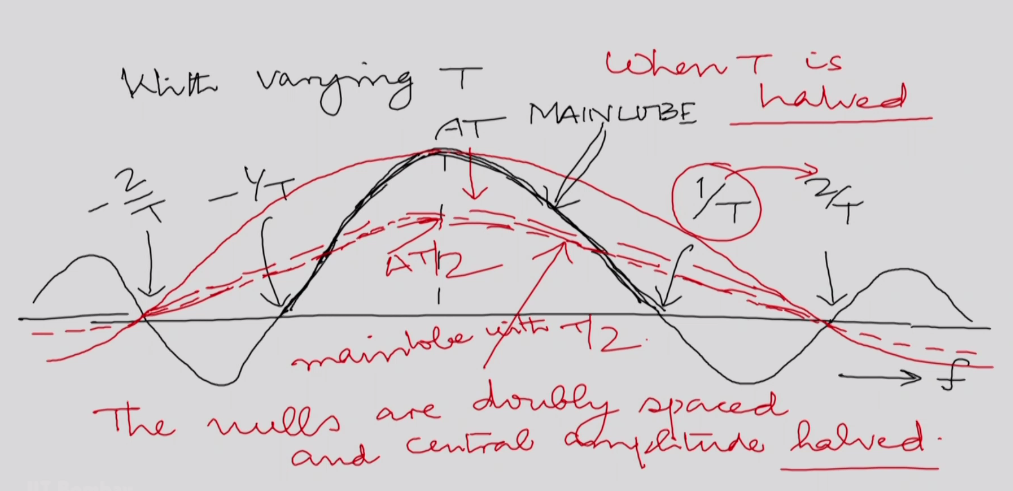
\includegraphics[width=12cm]{pulse_FT_half.png}
\caption{Fourier Transform of Rectangular Pulse at width T and T/2 }
\label{pulse_FT_half}
\end{figure}



\subsection{Properties of Fourier Transform}
When we change the signal in some way or when we bring signals together, what happens to the corresponding Fourier transform is what we will investigate in this section.

\subsubsection{Linearity}
Let $h_1(t)$ have the Fourier transform $H_1(\Omega)$ and let $h_2(t)$ have the Fourier transform $H_2(\Omega)$. Then, linearity says

%\begin{equation}
%$$\alpha h_1(t) + \beta h_2(t) \longrightarrow \alpha H_1(\Omega)+ \beta H_2(\Omega)$$
%\end{equation}


\[\alpha h_1(t) + \beta h_2(t) \xrightarrow{\mathfrak{F}} \alpha H_1(\Omega)+ \beta H_2(\Omega)\]
for all $\alpha$, $\beta$ $\in \mathbb{C}$ and all $h_1(t)$ and $h_2(t)$. Here, ${\mathfrak{F}}$ means ``has the Fourier transform given by".

\subsubsection{Proof of the linearity}
\begin{equation}
 \alpha \{ H_1(\Omega) \} = \alpha \{ \int_{-\infty}^{\infty} {h_1(t)e^{-j\Omega t}} dt \}
\label{one}
\end{equation}

\begin{equation}
 \beta \{ H_2(\Omega) \} = \beta \{ \int_{-\infty}^{\infty} {h_2(t)e^{-j\Omega t}} dt \}
\label{two}
\end{equation}

Add equation~\ref{one} and ~\ref{two}. We can write it as
\begin{equation}
\{ \alpha H_1(\Omega) + \beta H_2(\Omega) \} = \{ \int_{-\infty}^{\infty} {(\alpha h_1(t) + \beta h_2(t))e^{-j\Omega t}} dt \}
\end{equation}

\subsubsection{The Inverse Fourier transform}
Inverse Fourier transform can be written as
\begin{equation}
H_1(\Omega) \xrightarrow{\mathfrak{F}^{-1}} \frac{1}{2\pi} \int_{-\infty}^{\infty} {H_1(t)e^{j\Omega t}} d\Omega
\end{equation}

Note $\Omega$ = $2\pi f$, $d\Omega$= $2\pi df$

Whereupon
\begin{equation}
H_1(f) \xrightarrow{\mathfrak{F^-1}} \int_{-\infty}^{\infty} {H_1(f)e^{j2\pi ft}} df
\end{equation}

Where $\Omega$ =  Radians/sec frequency
And f = cycles/sec frequency

\begin{itemize}

\item We can clearly see that when frequency is in radians/sec then, we will have factor of $1/2\pi$ in the inverse Fourier transform and when frequency is in cycles/sec then the factor of $1/2\pi$ will not be there.
\item In a way dealing with cycles/second frequency has some conveniences, we don't need to remember the factor of $1/2\pi$ or we can say, there is a perfect symmetry between the Fourier transform and the Inverse Fourier transform.

\end{itemize}


\subsubsection{Exercise}
 Prove that \textbf{linearity} holds true for the inverse Fourier transform.



\subsection{Time Shift}
what happens to the Fourier transform when we shift the signal in time? If
\begin{equation}
h(t) \xrightarrow{\mathfrak{F}} H(\Omega)
\end{equation}
\noindent
then
\begin{equation}
h(t-\tau_0) \xrightarrow{\mathfrak{F}} {?}
\end{equation}
\noindent
So the Fourier transform would be
\begin{equation}
H(\Omega) =  \int_{-\infty}^{\infty} {h(t-\tau_0)e^{-j\Omega t}} dt
\end{equation}
Put $(t-\tau_0) = \lambda$  $\Rightarrow$  $t = \tau_0 + \lambda$.
So the Fourier transform is
\begin{equation}
H(\Omega) =  \int_{-\infty}^{\infty} {h(\lambda)e^{-j\Omega (\lambda + \tau_0)}} d\lambda =
e^{-j\Omega \tau_0}\int_{-\infty}^{\infty} {h(\lambda)e^{-j\Omega \lambda}} d\lambda
\end{equation}
\noindent
So,

\begin{equation}
h(t-\tau_0) \xrightarrow{\mathfrak{F}} e^{-j\Omega \tau_0} H(\Omega)\   or\   e^{-j2\pi f\tau_0} H(f)
\end{equation}
\noindent
Now it can be clearly seen that
\begin{itemize}
\item The magnitude of the Fourier transform is unchanged.
\item The angle or the phase of the Fourier transform changes.
\end{itemize}


\subsubsection{Modulation}
By modulation, we mean multiplying h(t) by a rotating complex number (rotating with an angular velocity of $\Omega_0$). In this case, the Fourier transform is shifted by $\Omega_0$ forward.

\begin{equation}
e^{j\Omega_0 t} h(t) \xrightarrow{\mathfrak{F}} {?}
\end{equation}
\noindent
So the Fourier transform would be
\begin{equation}
 \int_{-\infty}^{\infty} {e^{j\Omega_0 t}h(t)e^{-j\Omega t}} dt=
 \int_{-\infty}^{\infty} {h(t)e^{-j(\Omega-\Omega_0) t}} dt=
 H(\Omega-\Omega_0)
\end{equation}
\noindent
\begin{itemize}

\item When we shift a function in time, it causes a modulation in the frequency domain (We remember, it multiplied the Fourier transform by a term $e^{-j\Omega \tau_0}$).

\item When we modulate the function in time by multiplying by a rotating complex number, the corresponding Fourier transform shifts in frequency.

\item Basically, shift in time becomes modulation in frequency, and modulation in time becomes a shift in frequency.

\end{itemize}

\subsubsection{Convolution Property of Fourier transform}
The question to answer here is what will be the Fourier transform of $x_1(t)*x_2(t)$, given that the Fourier transforms of $x_1(t)$ and $x_2(t)$ are $X_1(\Omega)$ and $X_2(\Omega)$ respectively. 

\begin{equation}
x_1(t)\ast x_2(t) = \int_{-\infty}^{\infty}{x_1(\tau) x_2(t-\tau)}d\tau
\end{equation}

\begin{equation}
x_1(t)\ast x_2(t) \xrightarrow{\mathfrak{F}} {?}
\end{equation}
\noindent
Now let's solve it. The Fourier transform can be written as
\begin{equation}
\int_{-\infty}^{\infty} \{ \int_{-\infty}^{\infty} {x_1(\tau)x_2(t-\tau)} d\tau \} {e^{-j\Omega t}} dt
\end{equation}

This is same as
\begin{equation}
\int_{-\infty}^{\infty}\int_{-\infty}^{\infty} {x_1(\tau)x_2(t-\tau)e^{-j\Omega t}}d\tau dt
\end{equation}

To solve the above double integral we will do a change of variables. Put
\begin{equation}
\alpha =\tau \  and   \ \beta = (t-\tau)
\end{equation}

\begin{equation}
\left( \begin{array}{c}
\alpha \\
\beta \end{array} \right)
=
\left( \begin{array}{cc}
1 & 0 \\
-1 & 1 \end{array} \right)
\left( \begin{array}{c}
\tau \\
 t \end{array} \right)
\end{equation}

\begin{equation}
 \mathrm{d}\tau \mathrm{d}t = |\text{Det(transformation)}| \mathrm{d}\alpha \mathrm{d}\beta
\end{equation}
\noindent
Hence,
\begin{equation}
\mathrm{d}\tau \mathrm{d}t = \mathrm{d}\alpha \mathrm{d}\beta
\end{equation}
Hene, the element of integration also remains the same because the \textbf{jacobian} is $1$.
\noindent
Now the modified integral is
\[
\int_{-\infty}^{\infty}\int_{-\infty}^{\infty} x_1(\alpha)x_2(\beta) \exp{-j\Omega(\alpha+\beta)}d\alpha d\beta
\]
\begin{equation}
=\int_{-\infty}^{\infty} {x_1(\alpha) \{ \int_{-\infty}^{\infty}
{x_2(\beta)e^{-j\Omega(\beta)} d\beta }\} e^{-j\Omega \alpha}d\alpha }
\end{equation}
\noindent
This can be written as
\[
X_2(\Omega) \int_{-\infty}^{\infty} x_1(\alpha) e^{-j\Omega \alpha}d\alpha
\]
So
\begin{equation}
x_1(t)\ast x_2(t) \xrightarrow{\mathfrak{F}} X_1(\Omega)X_2(\Omega)
\end{equation}
\noindent
Hence a convolution in the natural domain moves to multiplication in the Fourier domain.


\subsection {Conclusion} In this lecture we discussed about Fourier transform of rectangular pulse which is the ``Sinc function'' and its properties. We showed some of the properties of Fourier transform and their proofs.






